\documentclass[ 12pt ]{article}
\usepackage{amsmath, amsthm, amssymb, csquotes, enumitem, graphicx, listings, mathrsfs}
\usepackage[margin=0.5in]{geometry}
\graphicspath{ ./ }

\begin{document}

\begin{titlepage}
    \begin{center}
        \vspace*{1cm}
            
        \LARGE
        \textbf{CS 479 Pattern Recognition}

        \vspace{0.5cm}
        \LARGE
        \textbf{Programming Assignment 1}

        \vspace{0.1cm}
        \LARGE
        \textbf{Bayesian Decision Theory}
            
        \vspace{1.5cm}
            
        \textbf{Logan Leavitt \& Landon Fox}
            
        \vfill
        \Large
        \textbf{Collaboration}

        \vspace{0.1cm}
        \large
        For the implementation, both Logan and Landon contributed. Logan carried out the Box-Muller transformation, the data set generation, and most debugging. Landon worked on the
        file input/output and active data classification. Together we collaborated on the various Bayesian classifiers. \\
        In regard to report, Logan worked on the Implementation, formatting, and grammar. Landon contributed to the Theory and Results.
            
        \vspace{0.8cm}
            
            
        \Large
        University of Nevada Reno\\
        March 10, 2021
            
    \end{center}
\end{titlepage}


\section*{Theory}

Bayesian decision theory studies the design of classifiers that make decisions using \textbf{Bayes rule}; that is, the field focuses on classifying a feature value $\textbf{x}$ into
a class $\omega_j$ using $$P(\omega_j|\textbf{x}) = \frac{P(\textbf{x}|\omega_j) P(\omega_j)}{P(\textbf{x})}.$$ Here, we say that $P(\textbf{x}|
\omega_j)$, $P(\omega_j)$, $P(\textbf{x})$, and $P(\omega_j|\textbf{x})$ are the likelihood, prior, evidence, and posterior, respectively. To determine if a feature $\textbf{x}$
belongs to a class $\omega_j$, then it likely holds that $P(\omega_j|\textbf{x}) = \sup_i P(\omega_i|\textbf{x})$. In other words, the likelihood that $\textbf{x}$ is a feature of
$\omega_j$ surpasses all others. We can further this idea by the use of a \textbf{discriminant}. A discriminant function is a function of $\textbf{x}$ that acts in a similar manner
to $P(\omega_j|\textbf{x})$ in a sense that we have a discriminant function for each class and that the maximum of them evaluated at $\textbf{x}$ illustrates the class most likely
to encompass $\textbf{x}$. Furthermore, it is easy to see that a discriminant function generalizes the notion of $P(\omega_j|\textbf{x})$ to better fit our purposes and simplify our
calculations, for instance. Particularly, if there are only two categories for which features can belong to, we may simplify our decision to
\begin{displayquote}
    choose $\omega_1$ if $g_1(\textbf{x}) - g_2(\textbf{x}) > 0$; otherwise choose $\omega_2$
\end{displayquote}
where $g_j(\textbf{x})$ is our discriminant function. Additionally, to determine precisely how our classifier would categorize a feature $\textbf{x}$, we can plot the \textbf{decision
boundary}, all points where $g_1(\textbf{x}) = g_2(\textbf{x})$, in Euclidean space to see which region $\textbf{x}$ belongs to.

When assuming that $P(\textbf{x}|\omega_j) \sim N(\mathbf{\mu}_j, \Sigma_j)$, a multivariable Gaussian distribution, and that we have the discriminant function $$g_j(x) = \ln P(\textbf{x}
|\omega_j) + \ln P(\omega_j),$$ a common and efficient model, we arrive at the model $$g_j(\textbf{x}) = -\frac{1}{2}(\textbf{x} - \mathbf{\mu}_j)^t \Sigma_j^{-1}(\textbf{x} -
\mathbf{\mu}_j) - \frac{d}{2} \ln 2\pi - \frac{1}{2} \ln |\Sigma_j| + \ln P(\omega_j)$$ where $d$ is the dimension of $\textbf{x}$ and $\textbf{mu}_j$. There are three major cases when
designing discriminants that all depend on the nature of $\Sigma_j$, the covariance matrix. In case one, we assume that $\Sigma_j = \sigma^2 I$ for all classes $j$. This is a proper
assumption only when all variables are uncorrelated and share the same variance, namely $\sigma^2$. Additionally, our discriminant functions are greatly simplified to $$g_j(\textbf{x})
= -\frac{||\textbf{x} - \mathbf{\mu}_j||^2}{2\sigma^2} + \ln P(\omega_j).$$ In fact, with the assumption that $$P(\omega_1) = P(\omega_2) = \hdots,$$ then we may further simplify our
model to $$g_j(\textbf{x}) = -||\textbf{x} - \mathbf{\mu}_j||^2,$$ the \textbf{Euclidean distance classifier}. Case two is quite similar to case one where we still use a single matrix
to model all classes, yet we ease the restriction that $\Sigma_j$ is a diagonal matrix. With this assumption, we obtain linear the discriminant $$g_j(\textbf{x}) = -\frac{1}{2}(
\textbf{x} - \mathbf{\mu}_j)^t \Sigma^{-1} (\textbf{x} - \mathbf{\mu}_j) + \ln P(\omega_j).$$ Finally, case three provides no restriction to $\Sigma_j$ for all classes. With no
restriction, we arrive at a quadratic discriminant, namely, $$g_j(\textbf{x}) = -\frac{1}{2}\textbf{x}^t \Sigma_j \textbf{x} + \mathbf{\mu}_j^t \left (\Sigma_j^{-1} \right )^t
\textbf{x} - \frac{1}{2}\mathbf{\mu}_j^t \Sigma_j^{-1} \mathbf{\mu}_j - \frac{1}{2} \ln |\Sigma_j| + \ln P(\omega_j).$$ When implementing a Bayesian classifier, it is vital to choose
the appropriate case as it could result in improper assumptions which may over simplify the model.

In regard to error, when using Gaussian distributions we can see that our error can be determined by $$P(\xi) = \int P(\xi, \textbf{x})\, \mathrm{d}\textbf{x} = \int P(\xi | \textbf{x})
P(\textbf{x})\, \mathrm{d}\textbf{x} = \int \min_j \{ P(\omega_j | \textbf{x}) \} P(\textbf{x})\, \mathrm{d}\textbf{x}.$$ Assuming that we have two classes and utilizing the fact that
$$\min \{ a, b \} \leq a^\beta b^{1-\beta},\;\;\; a, b \geq 0, 0 \leq \beta \leq 1,$$ we obtain $$P(\xi) = \int \min \{ P(\omega_1 | \textbf{x}), P(\omega_2 | \textbf{x}) \} P(\textbf{x}
)\, \mathrm{d}\textbf{x} \leq P^\beta(\omega_1) P^{1 - \beta}(\omega_2) \int P^\beta(\textbf{x} | \omega_1) P^{1 - \beta}(\textbf{x} | \omega_2)\, \mathrm{d}\textbf{x}.$$ It can be
further shown that $$\int P^\beta(\textbf{x} | \omega_1) P^{1 - \beta}(\textbf{x} | \omega_2)\, \mathrm{d}\textbf{x} = e^{-\kappa(\beta)}$$ where $$\kappa(\beta) = \frac{\beta(1 -
\beta)}{2}(\mathbf{\mu}_1 - \mathbf{\mu}_2)^t ((1- \beta)\Sigma_1 + \beta \Sigma_2)^{-1} (\mathbf{\mu}_1 - \mathbf{\mu}_2) + \frac{1}{2} \ln \frac{|(1 - \beta) \Sigma_1 + \beta
\Sigma_2|}{|\Sigma_1|^{1 - \beta} |\Sigma_2|^\beta}.$$ Hence, $$P(\xi) \leq P^\beta(\omega_1) P^{1 - \beta}(\omega_2) e^{-\kappa(\beta)}.$$ To further minimize the bound, we can minimize
the previous expression via $\beta$ to obtain the \textbf{Chernoff error bound}. Due to the fact that this can be computationally expensive, we may set $\beta = \frac{1}{2}$ to obtain a
simpler expression at the expense of precision. This bound is referred to as the \textbf{Bhattacharyya error bound}.

\section*{Implementation}

To implement our classifier for the given samples of the distributions, we require the use of three variants of Bayesian classifiers, particularly, we need an uncorrelated classifier
(case 1), an arbitrary classifier (case 3), and a Euclidean distance classifier. The file \verb|BayesianClassifer| is responsible for implementing the required aspects of all utilized
classifiers. A struct labeled \verb|Category| is responsible for containing all information regarding a class and its distribution such as the dimension of the space, \verb|dim|, the
center of the distribution, \verb|mu|, and other data of importance as seen below.
\begin{lstlisting}[basicstyle=\ttfamily\footnotesize, numbers=left, tabsize=4, frame=single]
struct Category
{
    unsigned int dim;
    std::vector<double> mu;
    std::vector<double> sigma;
    double prior;
    Category( unsigned int dim, std::vector<double> mu, std::vector<double> sigma,
        double prior );
};
\end{lstlisting}
Each classifier object will make use of precisely two categories for its classes. The class \verb|Classifier| acts as an abstract class inherited by the \verb|UncorrelatedClassifier|,
\verb|ArbitraryClassifier|, and \verb|EuclideanClassifier|.
\begin{lstlisting}[basicstyle=\ttfamily\footnotesize, numbers=left, tabsize=4, frame=single]
class Classifier {
public:
    Classifier(Category cat1, Category cat2);

    int classify(const std::vector<double> & x);

private:
    virtual double discriminant(const std::vector & x, int i) = 0;

    Category cat[2];
};
\end{lstlisting}
The method \verb|classify| makes use of \verb|discriminant| by taking the difference of the discriminant for each category, then returning the respective class the input vector \verb|x|
belongs to based on that result. The child classifiers each have their own implementation of their discriminant based on the assumptions used for the classifier. As an example,
\verb|EuclideanClassifer| returns the result $$-||\textbf{x} - \mathbf{\mu}_j||^2$$ evaluated at \verb|x|.

To obtain random samples of a Gaussian distribution, we use the polar Box-Muller transformation. Afterwards, we place all data into a CSV file. The respective CSV file is then read into
a vector, with the assistance of \verb|FileInput|, in the \verb|main| function of one of the following programs: \verb|problem1.cpp|, \verb|problem2.cpp|, \verb|problem3.cpp|,
\verb|problem4.cpp|. Then we instantiate the classifier associated with the problem and iterate through the input vector, classifying and recording the result each time.
\begin{lstlisting}[basicstyle=\ttfamily\footnotesize, numbers=left, tabsize=4, frame=single]
int main()
{
    std::vector< std::vector< double > > inputs      = read_csv( "test1.csv" );
    std::vector< std::vector< double > > inputs_temp = read_csv( "test2.csv" );
    int input1_len = inputs.size();
    inputs.insert( inputs.end(), inputs_temp.begin(), inputs_temp.end() );

    std::vector< double > mu1{ 1, 1 };
    std::vector< double > mu2{ 4, 4 };
    std::vector< double > sigma1{ 1, 1 };
    std::vector< double > sigma2{ 1, 1 };
    Category cat1( 2,  mu1, sigma1, 0.3 );
    Category cat2( 2,  mu2, sigma2, 0.7 );
    UncorrelatedClassifier classifier( cat1, cat2 );

    int misclassified1 = 0;
    int misclassified2 = 0
    std::ofstream file( "output.csv" );
    file << "x1, x2, Category" << std::endl;
    for ( int i = 0; i < inputs.size(); i++ )
    {
        int cat = classifier.classify( inputs[ i ] );
        if ( i < inputs1_len && cat == 2 )
            misclassified1++;
        else if ( i >= inputs1_len && cat == 1 )
            misclassified2++;
        file      << inputs[ i ][ 0 ] << ", " << inputs[ i ][ 1 ] << ", " << cat
            << std::endl;
        // std::cout << inputs[ i ][ 0 ] << ", " << inputs[ i ][ 1 ] << ", " << cat
            << std::endl;
    }
    file.close();
    std::cout << "Total misclassification rate : " << ( (double) ( misclassified1
            + misclassified2 ) / inputs.size() ) << '%' << std::endl
        << "Misclassification rate class 1 : " << ( (double) misclassified1
            / inputs.size() ) << '%' << std::endl
        << "Misclassification rate class 2 : " << ( (double) misclassified2
            / inputs.size() ) << '%' << std::endl;

    return 0;
}
\end{lstlisting}

\section*{Results}

\begin{enumerate}
    \item[\textbf{1.}]
        \begin{enumerate}
            \item[\textbf{a.}] Provided the Gaussian distributions $N(\mathbf{\mu}_1, \Sigma_1)$ and $N(\mathbf{\mu}_2, \Sigma_2)$ where $$\mathbf{\mu}_1 = \begin{bmatrix} 1 \\ 1
                \end{bmatrix},\; \Sigma_1 = \begin{bmatrix} 1 & 0 \\ 0 & 1 \end{bmatrix},\;\;\; \mathbf{\mu}_2 = \begin{bmatrix} 4 \\ 4 \end{bmatrix},\; \Sigma_2 = \begin{bmatrix} 1 & 0 \\
                0 & 1 \end{bmatrix},$$ belonging to data set $A$ we can see that the case one discriminant would be the most beneficial as $\Sigma_j = I_2$ for all $j$. Moreover, all
                random variables are uncorrelated and have the same value, in this case 1. Hence, case one would be the most simplified model suited for our classification. Provided that
                we know the distributions from which our samples are from and the precise amount from each, we can use this information to calculate the priors. Furthermore, $$P(\omega_1
                ) = \frac{60,000}{60,000 + 140,000} = \frac{3}{10},\;\;\; P(\omega_2) = \frac{140,000}{60,000 + 140,000} = \frac{7}{10}.$$ Otherwise, if we could not make this assumption,
                then we would assume uniform probability, that is $P(\omega_1) = P(\omega_2) = \frac{1}{2}$.

            \item[\textbf{b.}] Observe Figure 1 depicting data set $A$ along with the decision boundary $x+y = 5 + \frac{1}{3}\ln \frac{3}{7}$. We can see that large amounts of the data
                are properly divided where the blue region represents the first class and the orange region is the second class.
                \begin{center}
                    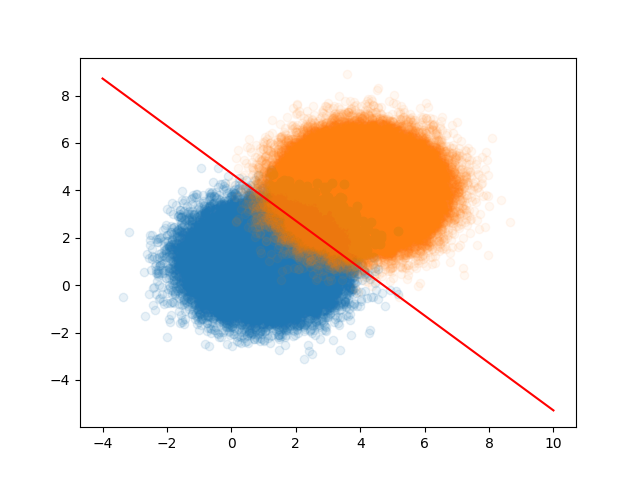
\includegraphics{figure1}
                    \scriptsize
                    Fig. 1: The plot of data set $A$ along with the decision boundary $x+y = 5 + \frac{1}{3}\ln \frac{3}{7}$.
                \end{center}

            \item[\textbf{c.}]
                \begin{enumerate}
                    \item[\textbf{i.}] After running the classification (\verb|program1.cpp|), we can see that the misclassification rate for class one is 0.008295\% and for class
                        two is 0.00719\%. We can see that each class has quite a low error.
                    \item[\textbf{ii.}] The total misclassification rate is 0.015485\%. Overall the classifier is working with high success.
                \end{enumerate}

            \item[\textbf{d.}] After computing the Bhattacharyya error bound, we obtain $\frac{\sqrt{21}}{10}e^{-9/4} = 4.8299992\%$. Observe that the result from \textbf{1c} is far
                lower than the result of the Bhattacharyya error. This may imply that the Bhattacharyya error is not the best error indicator for our specific model as our actual
                error is of two magnitudes lower. Moreover, the Chernoff error bound may be more well suited.
        \end{enumerate}

    \item[\textbf{2.}]
        \begin{enumerate}
            \item[\textbf{a.}] Provided the Gaussian distributions $N(\mathbf{\mu}_1, \Sigma_1)$ and $N(\mathbf{\mu}_2, \Sigma_2)$ where $$\mathbf{\mu}_1 = \begin{bmatrix} 1 \\ 1
                \end{bmatrix},\; \Sigma_1 = \begin{bmatrix} 1 & 0 \\ 0 & 1 \end{bmatrix},\;\;\; \mathbf{\mu}_2 = \begin{bmatrix} 4 \\ 4 \end{bmatrix},\; \Sigma_2 = \begin{bmatrix} 4 & 0 \\
                0 & 8 \end{bmatrix},$$ belonging to data set $B$ we can see that the case three discriminant would be the most beneficial as no restriction can be placed on $\Sigma_j$
                for all $j$ without over simplifying our model. Similar to \textbf{1a}, we obtain $$P(\omega_1) = \frac{40,000}{40,000 + 160,000} = \frac{1}{5},\;\;\; P(\omega_2) =
                \frac{160,000}{40,000 + 160,000} = \frac{8}{10}.$$

            \item[\textbf{b.}] Observe Figure 2 depicting data set $B$ along with the decision boundary $18 x^2 + 17 y^2 + 8 y = -32 - 8 \ln 2 - 65 \ln 5$. We can see that large amounts
                of the data are properly divided where the blue region represents the first class and the orange region is the second class.
                \begin{center}
                    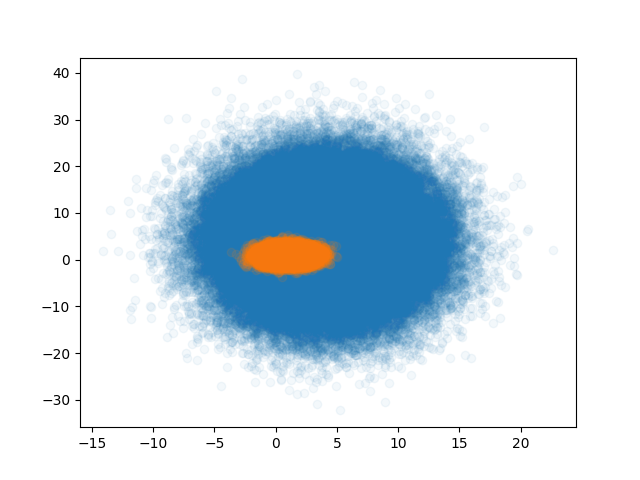
\includegraphics{figure2}
                    \scriptsize
                    Fig. 2: The plot of data set $B$ along with the decision boundary $18 x^2 + 17 y^2 + 8 y = -32 - 8 \ln 2 - 65 \ln 5$.
                \end{center}

            \item[\textbf{c.}]
                \begin{enumerate}
                    \item[\textbf{i.}] After obtaining our results from \verb|program2.cpp|, we can see that the misclassification rate for class one is 0.02746\% and for class
                        two is 0.04241\%. We can see that each class has quite a low error.
                    \item[\textbf{ii.}] The total misclassification rate is 0.06987\%. Overall the classifier is working with high success.
                \end{enumerate}

            \item[\textbf{d.}] After computing the Bhattacharyya error bound, we obtain $\frac{8 \sqrt[4]{2}}{15 \sqrt{5}} e^{-7/10} = 14.0852671\%$. Similar to \textbf{1d}, we can see
                that our actual error is far less than the Bhattacharyya error, again implying that it may not be a tight bound for our model.
        \end{enumerate}

    \item[\textbf{3.}] The misclassification rate for class one and class two are 0.004975\% and 0.011855\% respectively, providing a total misclassification rate of 0.01683\%. Observe that the rate for class one is better than the rate of the case one classifier. However, observe that it is not the case for class two; it far exceeds its error. Furthermore, the Euclidean classifier favors class two. This is because the Euclidean classifier is making the assumption that $P(\omega_1) = P(\omega_2)$.

    \item[\textbf{4.}] The misclassification rate for the Euclidean classifier on dataset B is given by 0.00342\% for class 1, 0.29557\% for class 2, and a total misclassification rate of 0.29899\%. One can see the classifier is misclassifying a larger number of elements from class 2 as class 1 elements. This shows the failure of the Euclidean Distance classifier to take into account the variance of each class, as well as their priors, $P(\omega_1)$ and $P(\omega_2)$. Compared to the misclassification rates given in (2.), this classifier is far from optimal, given these two datasets.

\end{enumerate}


\end{document}



